\hypertarget{missioneditor}{\section{Missions-Editor}}

\begin{figure}[H]
	\centering
	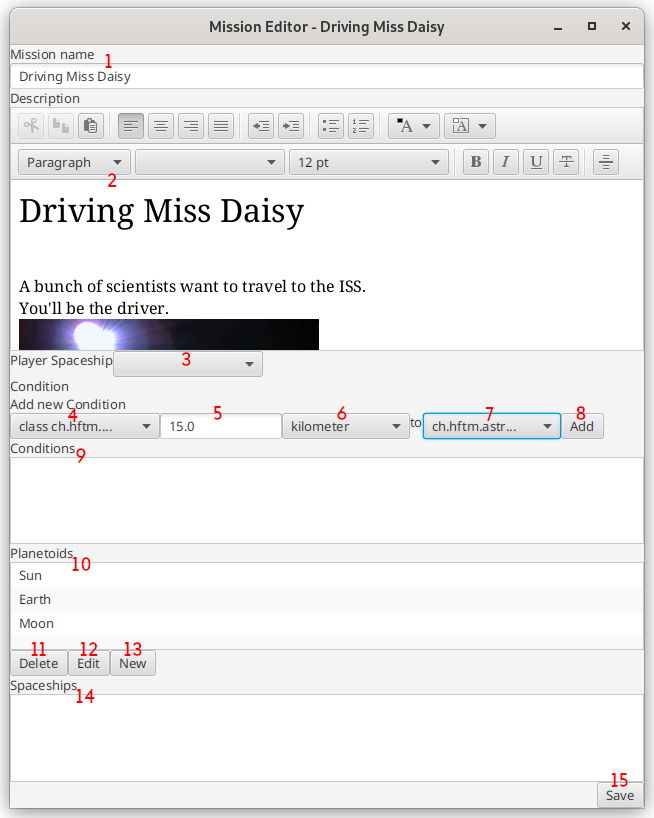
\includegraphics[width=12cm]{res/missioneditor.png}
	\caption{GUI Mission-Editor mit Annotation. Testmission 'Driving Miss Daisy' geöffnet.}
\end{figure}

\begin{enumerate}[noitemsep]
	\item Missionsname
	\item Missionsbeschreibung HTML-Editor
	\item Auswahl Spielerraumschiff
	\item Missionsbedingung: Bedingungstyp-Dropdown
	\item Missionsbedingung: Zahlenfeld
	\item Missionsbedingung: Masseinheit-Dropdown
	\item Missionsbedingung: Referenzobjekt-Dropdown
	\item Missionsbedingung hinzufügen
	\item Missionsbedingungen-Liste
	\item Planetoiden-Liste
	\item Planetoid entfernen
	\item Planetoid editieren
	\item Planetoid hinzufügen
	\item Raumschiff-Liste
	\item Missionsänderungen speichern
\end{enumerate}

\subsection{Grundlagen}
Der Missions-Editor erlaubt das Ändern des Missions-Namen und Beschreibung. Durch das Hinzufügen von Missionsbedingungen, auch Conditions genannt, können Abbruchsbedinungen für die Simulation festgelegt und weitere dynamische Veränderungen an der Mission vorgenommen werden. Verwendete Planetoiden und Raumschiffe werden in den ensprechenden Listen aufgelistet.

\hypertarget{addcondition}{\subsection{Hinzufügen einer Missionsbedingung}}
Wählen sie im Bedingungstyp-Dropdown den passenden Bedingungstypen.
Siehe \hyperlink{conditiontable}{Abschnitt Missionsbedingen} für eine komplette Liste der möglichen Bedingungstypen, ihren Parametern, und Funktionsweise.
Zahlenfeld, Grössenangabe und Referenzobjekt werden dynamisch ein- oder ausgeblendet.

% nifty way to make two figures side by side
\begin{figure}[H]
	\centering
	\begin{minipage}[b]{0.45\textwidth}
		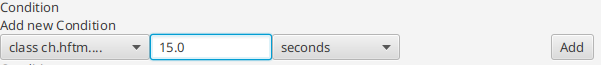
\includegraphics[width=\textwidth]{res/conditionmaxtime.png}
		\caption{MaximumTime}
	\end{minipage}
	\hfill
	\begin{minipage}[b]{0.45\textwidth}
		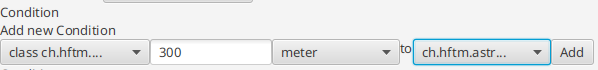
\includegraphics[width=\textwidth]{res/conditionapproach.png}
		\caption{Approach}
	\end{minipage}
\end{figure}

Sollte das Zahlenfeld oder das Referenzobjekt eingeblendet werden so ist eine Eingabe respektive Auswahl zwingend.
Die Masseinheit kann jederzeit geändert werden, ein valider Wert im Zahlenfeld wird in die neue Einheit umgewandelt.

\begin{figure}[H]
	\centering
	\begin{minipage}[b]{0.45\textwidth}
		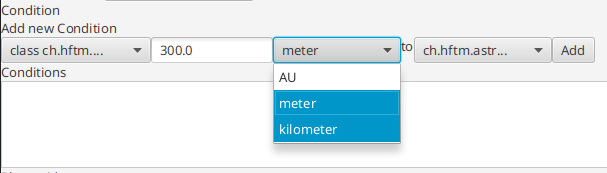
\includegraphics[width=\textwidth]{res/conditionunits.png}
		\caption{Masseinheit Meter}
	\end{minipage}
	\hfill
	\begin{minipage}[b]{0.45\textwidth}
		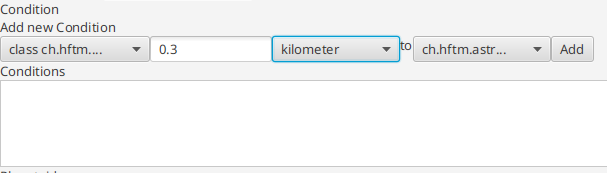
\includegraphics[width=\textwidth]{res/conditionunits2.png}
		\caption{Masseinheit Kilometer}
	\end{minipage}
\end{figure}

Klicken sie auf den Add-Button um die Missionsbedingung hinzuzufügen.
Die Missionsbedingung wird nun in der Missionsbedingungen-Liste aufgeführt.

\begin{figure}[H]
	\centering
	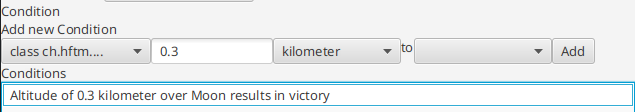
\includegraphics[width=0.45\textwidth]{res/conditionadded.png}
	\caption{Neue Approach-Missionsbedingung hinzugefügt}
\end{figure}

\hypertarget{conditiontable}{\subsection{Missionsbedingungen}}

\begin{table}[H]
	\centering
	\begin{tabular}{ || m{3cm} | m{5cm} | m{8cm} || }
		\hline
		\textbf{Bedingung} & \textbf{Parameter} & \textbf{Funktionsweise} \\
		\hline
		\hline
		MaximumTime & Zeitwert & Mission gilt als Fehlschlag wenn Missionsdauer den Zeitwert überschreitet \\
		\hline
		HoldoutTime & Zeitwert & Mission gilt als Gewonnen wenn Missionsdauer den Zeitwert überschreitet \\
		\hline
		Approach & Distanz und Referenzobjekt & Mission gilt als Gewonnen wenn Spielerraumschiff die maximale Distanz zum Referenzobjekt erreicht oder unterschreitet \\
		\hline
		Avoid & Distanz und Referenzobjekt & Mission gilt als Fehlschlag wenn Spielerraumschiff die maximale Distanz zum Referenzobjekt erreicht oder unterschreitet \\
		\hline
		Depart & Distanz und Referenzobjekt & Mission gilt als Gewonnen wenn Spielerraumschiff die minimale Distanz zum Referenzobjekt erreicht oder überschreitet \\
		\hline
		SetupHeavyLander & Distanz und Referenzobjekt & Platziert das Raumschiff 'Heavy Lander' in ein Orbit um Referenzobjekt mit Höhe von Distanz\\
		\hline
		SetupISS & Distanz und Referenzobjekt & Platziert das Raumschiff 'ISS' in ein Orbit um Referenzobjekt mit Höhe von Distanz\\
		\hline
	\end{tabular}
	\caption{Verfügbare Missionsbedingungem}
\end{table}

\subsection{Löschen eines Planetoiden}
Wählen sie den zu löschenden Planetoiden mit einem Klick aus der Planetoiden-Liste aus.
Klicken sie den Delete-Button.
Es öffnet sich eine Sicherheitsabfrage.

\begin{figure}[H]
	\centering
	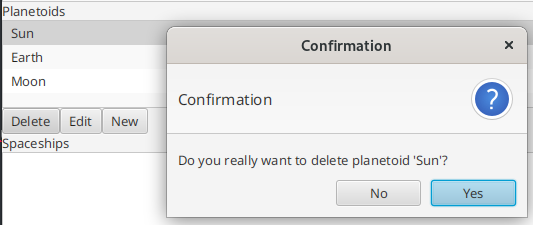
\includegraphics[width=0.45\textwidth]{res/loeschenplanetoid.png}
	\caption{Sicherheitsabfrage bei Planetoidenlöschung}
\end{figure}

Bestätigen sie das Popup mit Yes.
Der Planetoid ist nun aus der Mission entfernt und die Planetoiden-Liste aktualisiert worden.

\subsection{Editieren eines Planetoiden}
Wählen sie den zu editierenden Planetoiden mit einem Klick aus der Planetoiden-Liste aus.
Klicken sie auf den Edit-Button.
Es öffnet sich nun der Planetoid-Editior mit dem ausgewählten Planetoiden.
Für Details zum Planetoid-Editior konsultieren sie das \hyperlink{planetoideditor}{Kapitel Planetoid-Editior}.

\subsection{Hinzufügen eines Planetoiden}
Klicken sie auf den New-Button unterhalb der Planetoiden-Liste.
Es öffnet sich nun der Planetoid-Editior.
Für Details zum Planetoid-Editior konsultieren sie das \hyperlink{planetoideditor}{Kapitel Planetoid-Editior}.

\subsection{Hinzufügen eines Raumschiffs}
Zum hinzufügen eines Raumschiffs benutzen sie die Condition 'SetupHeavyLander'.
Siehe \hyperlink{addcondition}{Abschnitt Hinzufügen einer Missionsbedingung}.